
The optimality of sparse signal detection was first studied by \citet{ingster1998minimax}, who showed that a phase transition in the $r$-$\beta$ plane exists for the signal detection problem. 
Specifically, consider the so-called {\em detection boundary} function:
\begin{equation} \label{eq:detection-boundary-large-signals}
    f(\beta) = 
    \begin{cases}
        \max\{0,\beta -1/2\} & 0<\beta\le 3/4\\
        \left(1 - \sqrt{1-\beta}\right)^2 & 3/4 < \beta \le 1.
    \end{cases}
    \quad\quad \beta\in (0,1].
\end{equation} 
Assume that the non-zero signal sizes are all equal and parameterized as $\sqrt{2{r}\log{p}}$.
If the signal size parameter $r$ is {\em above} the detection boundary, i.e., $r>f(\beta)$, then the global null 
hypothesis $\mu(i)=0$ for all $i=1,\dots,p$ can be distinguished from the alternative as $p\to\infty$ in the sense of \eqref{eq:support-recovery-success} using the likelihood ratio test.  Otherwise, when the signal sizes fall below the boundary, i.e., $r< f(\beta)$, no test can do better than a 
random guess.  We visualize the detection boundary in the upper panel of Figure
\ref{fig:phase-diagram-signal-detection}.

Adaptive tests such as Tukey's \ac{HC} in \eqref{eq:HC-statistic} \citep{donoho2004higher} and a modified 
goodness-of-fit test statistic of \citet{zhang2002powerful} have been identified to attain this performance limit 
without knowledge of the sparsity and signal sizes. It is also known that the max-statistic \eqref{eq:max-statistic} is only efficient when $r>(1+\sqrt{1-\beta})^2$, and is therefore sub-optimal for denser signals where $1/2\le\beta\le 3/4$; see \cite{cai2011optimal}.
In contrast, the sum-of-square-type statistics such as $L_2$ was shown in \cite{fan1996test} to be asymptotically powerless when the $L_2$-norm of the signal $\|\mu\|_2^2$ is $o(\sqrt{p})$, or equivalently, when $\beta>1/2$ in our parametrization.

Notice that the scaling for the signal magnitude $\Delta = \sqrt{2r\log{p}}$ is useful for studying very sparse signals ($\beta>1/2$), but fails to reveal the difficulties of the detection problems when the signals are relatively dense 
($\beta<1/2$).  This is because $f(\beta) = 0,\ \beta\in (0,1/2]$. Thus, a different scaling is needed to study the regime of
small but dense signals.  In this case, with slight overloading of notation, we parametrize signal sizes as 
\begin{equation} \label{eq:signal-size-small} 
    \underline{\Delta} = p^{\underline{r}}
    \le \mu(i) \le
    \overline{\Delta} = p^{\overline{r}}, \quad \text{for all}\;\;i\in S_p,
\end{equation}
where $\underline{r}$ and $\overline{r}$ are {\rm negative} constants and 
the signal magnitude vanishes, as $p\to\infty$.
In this scaling, for the so-called faint signal regime, \citet{cai2011optimal} established a phase 
transition result characterized by the following boundary,
\begin{equation} \label{eq:detection-boundary-small-signals}
    f_s(\beta) = \beta - 1/2, \quad 0 < \beta \le 1/2.
\end{equation} 
Specifically, if $\overline{r}<f_s(\beta)$, the signal detection fails in the sense of \eqref{eq:support-recovery-failure} regardless of the procedures, while the \ac{HC} statistic continues to attain asymptotically perfect detection when $\underline{r}>f_s(\beta)$. 
We visualize this boundary in the lower panel of Figure \ref{fig:phase-diagram-signal-detection}.

\begin{figure}
      \centering
      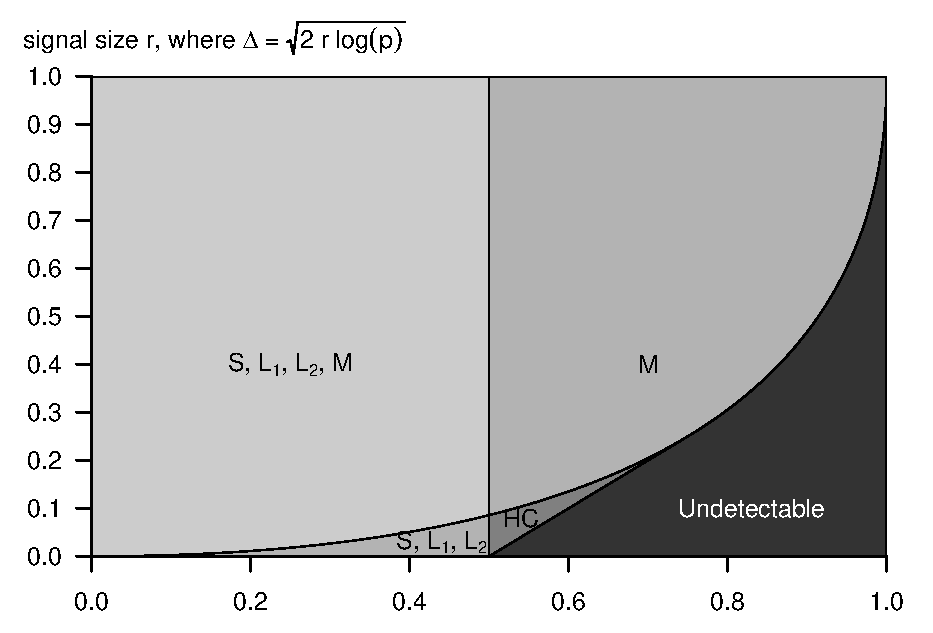
\includegraphics[width=0.7\textwidth]{figures/phase_diagram_signal_detection.eps}
      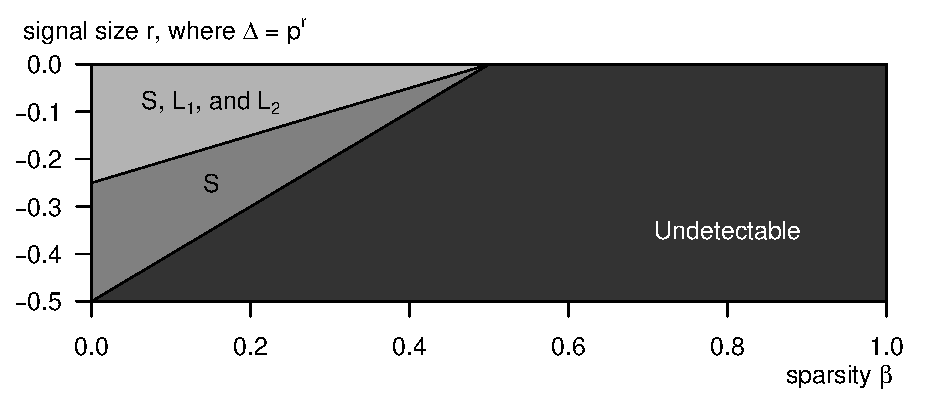
\includegraphics[width=0.7\textwidth]{figures/phase_diagram_signal_detection_vanishing_signals.eps}
      \caption{The phase diagrams of the sparse signal detection problem. 
      Signal size and sparsity are parametrized by $r$ and $\beta$, respectively.
      % Signal sparsity $|S|$ is parametrized by $\beta$. 
      % Signal sizes $\Delta$, parametrized by $r$, increases with dimension $p$ inside the upper panel, and decreases with $p$ inside the power panel.
      The diagrams illustrate the regions where the signal detection problem can be solved asymptotically by some of the commonly used statistics: the maximum ($M$), the sum-of-squares ($L_2$), the sum-of-absolute values ($L_1$), and the sum ($T$).
      In each region of the diagram, the annotated statistics can make the detection risk \eqref{eq:risk-detection} vanish, as dimension $p$ diverges. Conversely, the risks has liminf at least one.
      The detection problem is unsolvable for very sparse and weak signals in the undetectable regions.
      Notice that the $L_1$ and $L_2$ statistics are in fact sub-optimal for all sparsity levels.
      On the other hand, the max-statistic remains powerful for sparse signals ($\beta>1/2$), and is fully efficient when the problem is very sparse ($\beta\ge3/4$).
      The \ac{HC} statistic can detect signals in all configurations in the detectable regions.
      See text and Theorem \ref{thm:detection-optimality}.}
      \label{fig:phase-diagram-signal-detection}
\end{figure}


To the best of our knowledge, performance of simple statistics such as $L_1$, $L_2$ norms, and 
\stilian{the sum statistic $T$ in \eqref{eq:sum-statistic}}{R2, Typo 7}
in this weak signal setting have not been reported in the literature. %perhaps due to a perceived lack of novelty. 
Our first theorem establishes the performance of these simple but popular statistics for detecting sparse signals 
in high-dimensions, and summarizes the known results.

\begin{theorem} \label{thm:detection-optimality}
Consider the signal detection problem in the triangular array of Gaussian error models \eqref{eq:model-additive-Chapter3} where the sparsity is parametrized as in \eqref{eq:signal-sparsity-additive}.
\begin{itemize}
    \item For signals whose sizes are parametrized as in \eqref{eq:signal-size-additive}, the detection problem can be asymptotically solved in the sense of \eqref{eq:support-recovery-success} with $L_2$, $L_1$, or $S$ statistic when $\beta\le 1/2$; on the other hand, these statistics are asymptotically powerless in the sense of \eqref{eq:support-recovery-failure} when $\beta>1/2$.
    \item For small and dense signals whose signal sizes are parametrized as in \eqref{eq:signal-size-small}, the detection problem can be asymptotically solved in the sense of \eqref{eq:support-recovery-success} with $L_2$ or $L_1$ statistic when $\underline{r}>\beta/2-{1}/{4}$; on the other hand, these statistics are asymptotically powerless in the sense of \eqref{eq:support-recovery-failure} when $\overline{r}<\beta/2-{1}/{4}$.
    Further, tests based on the $S$ statistic can succeed asymptotically in the sense of \eqref{eq:support-recovery-success} when $\underline{r}>\beta-1/2$, hence attaining the boundary of detectability in \eqref{eq:detection-boundary-small-signals}.
\end{itemize}
\end{theorem}

Theorem \ref{thm:detection-optimality} is proved in Section \ref{sec:supplement}.
We visualize the results in Theorem in Figure \ref{fig:phase-diagram-signal-detection}.
It is worth noting that the $\beta$-$r$ parameter regions where $L_1$ and $L_2$ statistics are asymptotically powerful coincide, and these statistics are theoretically suboptimal for both sparse regimes ($\beta>1/2$) and relatively dense regimes ($\beta\le 1/2$).

Ideas have been proposed to combine statistics that are powerful for different alternatives to create adaptive tests that maintain high power for at all sparsity levels.
Such adaptive tests can be constructed, for example, by leveraging the asymptotic independence of the sum- and supremum-type statistics \citep{hsing1995note}. 
Recently, \citet{xu2016adaptive} showed that for dependent observations under mixing and moment conditions, the sum-of-power-type statistics
\begin{equation}
    \widetilde{L}_q(x) = \sum_{i=1}^p x^q(i)
\end{equation} 
with distinct positive integer powers (i.e., $q=1,2,\ldots$) are asymptotically jointly independent, and proposed an adaptive test that monitors the minimium p-value of tests constructed with $\tilde{L}_q$'s.
This idea is further developed in \cite{wu2019adaptive} for generalized linear models and in \cite{he2018asymptotically} with U-statistics.

Optimality properties of such adaptive tests and the optimal choice of the $q$-combinations, however, remain open problems.
\cite{xu2016adaptive} suggested combine $q=1, 2, 3, \ldots, 6$, and  $q=\infty$, based empirical evidence from numerical experiments. 
Theorem \ref{thm:detection-optimality} here implies that, at least for detecting one-sided alternatives, the $\widetilde{L}_2$ statistic (i.e., $L_2$ norm) and the $L_1$ norm are asymptotically dominated by the $\widetilde{L}_1$ statistic (or equivalently, the sum $S$). Therefore it is sufficient to include only the latter in the construction of the adaptive test. 







